% Auriga theme
% https://github.com/anishathalye/auriga

\documentclass[14pt,aspectratio=169]{beamer}
\usepackage{pgfpages}
\usepackage{fancyvrb}
\usepackage{booktabs,dcolumn}
\usepackage{tikz}
\usetikzlibrary{arrows.meta, positioning, quotes}
\usepackage{pgfplots}

% \ifnotes
% \setbeamertemplate{note page}[plain]
% \setbeameroption{show notes on second screen=right}
% \fi

\usetheme{auriga}
\usecolortheme{auriga}

% define some colors for a consistent theme across slides
\definecolor{red}{RGB}{181, 23, 0}
\definecolor{blue}{RGB}{0, 118, 186}
\definecolor{gray}{RGB}{146, 146, 146}

\title{Historia Económica Argentina}

\author{\underline{Sebastián Freille} \inst{1}}

\institute[shortinst]{\inst{1} IEF-UNC \\ UCC}
\date{}

\AtBeginSection[]{
    \begin{frame}
    \vfill
    \centering
    \begin{beamercolorbox}[sep=8pt,center,shadow=true,rounded=true]{title}
        \usebeamerfont{title}\insertsectionhead\par%
    \end{beamercolorbox}
    \vfill
    \end{frame}
}



\AtBeginSubsection[]{
    \begin{frame}
    \vfill
    \centering
    \begin{beamercolorbox}[sep=6pt,center,shadow=true,rounded=true]{title}
        \usebeamerfont{title}\insertsubsectionhead\par%
    \end{beamercolorbox}
    \vfill
    \end{frame}
}


\AtBeginSubsubsection[]{
    \begin{frame}
    \vfill
    \centering
    \begin{beamercolorbox}[sep=4pt,center,shadow=true,rounded=true]{title}
        \usebeamerfont{title}\insertsubsubsectionhead\par%
    \end{beamercolorbox}
    \vfill
    \end{frame}
}


\begin{document}

{
  % rather than use the frame options [noframenumbering,plain], we make the
  % color match, so that the indicated page numbers match PDF page numbers
  \setbeamercolor{page number in head/foot}{fg=background canvas.bg}
  \begin{frame}
    \titlepage
  \end{frame}
}

  
  \section{Capítulo 1. El período de progreso}

  \subsection{Sistema de Bancos Nacionales Garantidos}


  \begin{frame}\frametitle{Bancos Nacionales Garantidos}
    \begin{itemize}\itemsep 10pt
      \item Hacia fines de 1887 se sancionó la Ley de Bancos
        Nacionales Garantidos (``sistema de banca libre'') 
\item El sistema funcionaba otorgando la libertad de emitir papel
  moneda a cualquier banco existente/nuevo con el requisito de comprar
  bonos públicos en oro
  \item Varios requisitos $\longrightarrow$ 1)
    capital inicial (250 mil); 2) reserva requerida del 10\% emisión;
    3) bonos \textit{nuevos} creados pagados con oro con un descuento
    del 15\%; 4) daban interés anual del 4.5\%; 5) había tope de
    emisión (90\% de 250 mil para cada banco, 40 millones total)
  \end{itemize}
      \end{frame}


     \begin{frame}\frametitle{}
       \begin{block}{Un ejemplo}
Un banco que quiera recibir 100 pesos moneda nacional en billetes debía depositar 85 pesos
oro en el Banco Nacional y a cambio recibía un bono público de 100
pesos oro. De los 100 en billetes recibidos debia inmoviliar 10 como
reservas. Solo 90 pesos moneda nacional en billetes entrarían en
circulación (pasivo) a cambio de operaciones comerciales del banco
--comprar mas oro, créditos/descuentos, aumentar reservas
bancarias. Dado que el oro se compraba a una prima de 35\% sobre el
papel, el banco necesitaba de 115 pesos papel para poner en
circulación 90 --25 pesos quedaban inmovilizados sin ganar interés.
         \end{block}
       \end{frame}


       \begin{frame}\frametitle{Bancos Nacionales Garantidos (cont.)}
\begin{figure}[htbp]\vspace{0cm}
  \centering
  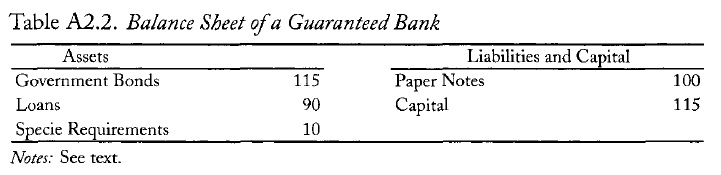
\includegraphics[scale=0.75]{uni1_mon14}
  \caption[bpe]{Hoja de balance de un banco garantido. Fuente: Della
    Paolera y Taylor (1992)}
  \label{fig:uni1_01}
\end{figure} 
  \end{frame}



   \begin{frame}\frametitle{Bancos Nacionales Garantidos (cont.)}
    \begin{itemize}\itemsep 10pt
      \item Rentabilidad bancaria dada por
        varios factores --$NPV$ valor presente neto, $B$ valor pesos
        papel bono, $PAR$ valor nominal bono,
        $R$ interes anual bono, $N$ tamaño de emision neta de reservas, $i$ retorno de activos alternativos
        \begin{equation*}
          NPV=-B+\sum_{t=1}^{T}\frac{iN+R}{(1+i)^{t}}+\frac{PAR}{(1+i)^{t}}
        \end{equation*}
      \item Si $T$ es grande, la medida de rentabilidad es:
        \begin{equation*}
          NPV=-B+\frac{(iN+R)}{i}=(N-B)+(R/i)
        \end{equation*}
        \item La emisión será rentable --$NPV>0$- si $R/(B-N)>i$          
           \end{itemize}
      \end{frame}




        \begin{frame}\frametitle{Bancos Nacionales Garantidos (cont.)}
    \begin{itemize}\itemsep 10pt
      \item Si el ratio entre los intereses de los bonos públicos y el
        capital inmovilizado por el banco era mayor a la tasa de
        retorno en activos alternativos, entonces convenía ser un un
        banco nacional garantido
        \item Suponiendo que el tipo de cambio peso oro/peso papel sea
          de 1.35, los bonos pagaban 4.5\% de interes entonces el
          interés por 100 pesos oro de bono era de 6.075; $R/(B-N)$
          por tanto era igual 24.4\% --bastante por encima de la tasa
          de retorno de inversiones alternativas.
          \item Si la inversión era rentable $\longrightarrow$ ¿por qué tardaron en
          entrar bancos privados?
           \end{itemize}
      \end{frame}



      

        \begin{frame}\frametitle{Bancos Nacionales Garantidos (cont.)}
    \begin{itemize}\itemsep 10pt
      \item Tanto los bancos oficiales (públicos/mixtos) como los
        bancos privados no usaron en general capital pre-existente
        para comprar los bonos (derecho a emisión) sino que
        contrajeron deuda en Londres --operación de arbitraje. La
        inversión era rentable si:
        \begin{equation}
i^{*}B<iN+R
          \end{equation}
\item Cuando luego se levantó el requisito del bono público, hubo una
  explosión de ``banca salvaje'' (\textit{wildcat
    banking}). Recordemos que $N-B$ era negativo (bono valía 115 pesos
  y le emision neta era de 90 pesos)
        \end{itemize}
      \end{frame}
    


      
        \begin{frame}\frametitle{Bancos Nacionales Garantidos (cont.)}
    \begin{itemize}\itemsep 10pt
    \item En ese caso, tenemos que:
      \begin{equation*}
(N-B)>0
         \end{equation*}
\item En otras palabras, el precio pagado por el derecho a emitir (el
  precio de compra de los bonos) era menor al valor de los billetes emitidos
\item Como consecuencia los bancos ``sobre-emitieron'' --evidencia de
  que solo el 50\% de los bonos adquiridos por los bancos fueron
  pagados en oro
\end{itemize}
      \end{frame}
    

  \begin{frame}\frametitle{Bancos Nacionales Garantidos (cont.)}
\begin{figure}[htbp]\vspace{0cm}
  \centering
  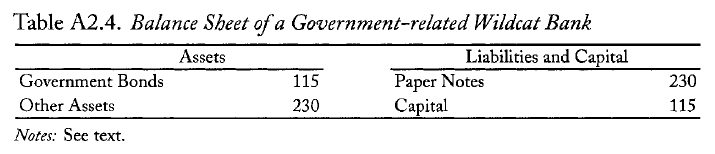
\includegraphics[scale=0.75]{uni1_mon15}
  \caption[bpe]{Hoja de balance de un banco garantido ``salvaje''. Fuente: Della
    Paolera y Taylor (1992)}
  \label{fig:uni1_01}
\end{figure} 
  \end{frame}

      

      
        \end{document}

        